%FIXME add a house as an example for transformation
\chapter{Matrices as Transformations}
Recall that a \emph{function}, informally, is a rule that takes an input and produces an output. 

For example, we know the common function $f(x) = x^3$ takes the input and cubes it, such that the result is $x \times x \times x$. Inputting $x=3$ outputs $f(3) = 27$. 

In Linear Algebra, we can think of matrices as a type of function. Recall our systems of matrices equation,
$$A\vec{x}=\vec{b}$$
We can rearrange this to look closer to function notation:
$$\vec{b}=A\vec{x}$$
We can change our input vector $\vec{x}$, which directly affects the output variable $\vec{b}$. 

Recall our subspace diagram; the matrix $A$, which is size $m\times n$, takes the input vectors $\vec{x} \in \mathbb R^n$, and transforms them to the output $\vec{b} \in \mathbb R^m$.


The transformation $T$ is said to map from the reals of $n$ to the reals of $m$, such that: $T: \mathbb R^{n}\to \mathbb R^m$
\begin{itemize}
    \item $\mathbb R^n$ is called the \textbf{domain}
    \item $\mathbb R^m$ is called the \textbf{codomain}
\end{itemize}

\begin{figure}[H]
    \centering
    %drawing made in mathcha 
    \tikzset{every picture/.style={line width=0.75pt}} %set default line width to 0.75pt        

    \begin{tikzpicture}[x=0.75pt,y=0.75pt,yscale=-1,xscale=1]
    %uncomment if require: \path (0,300); %set diagram left start at 0, and has height of 300

    %Curve Lines [id:da9612466263999061] 
    \draw    (106,59) .. controls (145.6,29.3) and (213.62,28.02) .. (252.82,58.08) ;
    \draw [shift={(254,59)}, rotate = 218.48] [color={rgb, 255:red, 0; green, 0; blue, 0 }  ][line width=0.75]    (10.93,-3.29) .. controls (6.95,-1.4) and (3.31,-0.3) .. (0,0) .. controls (3.31,0.3) and (6.95,1.4) .. (10.93,3.29)   ;
    %Curve Lines [id:da47200980654646296] 
    \draw    (106.47,82.73) .. controls (139.39,120.02) and (217.54,120.4) .. (253,81) ;
    \draw [shift={(105,81)}, rotate = 50.63] [color={rgb, 255:red, 0; green, 0; blue, 0 }  ][line width=0.75]    (10.93,-3.29) .. controls (6.95,-1.4) and (3.31,-0.3) .. (0,0) .. controls (3.31,0.3) and (6.95,1.4) .. (10.93,3.29)   ;


    % Text Node
    \draw (108.96,68) node  [xscale=0.8,yscale=0.8]  {$\mathbb{R}^{n}$};
    % Text Node
    \draw (255.96,68) node  [xscale=0.8,yscale=0.8]  {$\mathbb{R}^{m}$};
    % Text Node
    \draw (94,59) node [anchor=east] [inner sep=0.75pt]  [xscale=0.8,yscale=0.8]  {$N( A)$};
    % Text Node
    \draw (94,79) node [anchor=east] [inner sep=0.75pt]  [xscale=0.8,yscale=0.8]  {$R( A)$};
    % Text Node
    \draw (271.87,59) node [anchor=west] [inner sep=0.75pt]  [xscale=0.8,yscale=0.8]  {$N\left( A^{\top }\right)$};
    % Text Node
    \draw (272.81,79) node [anchor=west] [inner sep=0.75pt]  [xscale=0.8,yscale=0.8]  {$C( A)$};
    % Text Node
    \draw (178.9,19.84) node  [xscale=0.8,yscale=0.8]  {$\underset{m\times n}{A}$};
    % Text Node
    \draw (176.9,127.84) node  [xscale=0.8,yscale=0.8]  {$\underset{n\times m}{A^{\top }}$};
    % Text Node
    \draw (139,119) node [anchor=east] [inner sep=0.75pt]  [xscale=0.8,yscale=0.8]  {$ \begin{array}{l}
    N( A) \ \perp \ R( A)\\
    N( A) \ \cdot \ R( A) \ =\ 0
    \end{array}$};
    % Text Node
    \draw (371,122) node [anchor=east] [inner sep=0.75pt]  [xscale=0.8,yscale=0.8]  {$ \begin{array}{l}
    N\left( A^{\top }\right) \ \perp \ C( A)\\
    N\left( A^{\top }\right) \ \cdot \ C( A) \ =\ 0
    \end{array}$};


    \end{tikzpicture}
    \label{fig:transformationDiagram}
\end{figure}

Let's call the transformation $T$, such that 
$$T : \mathbb R^n \to \mathbb R^m$$

We can rewrite our transformation with matrix $A$ 
$$T(\vec x) = A\vec x$$

A matrix transformation is completely determined by where it sends the \emph{standard basis vectors}. Each column of $A$ is the image of a basis vector under the transformation, and every output vector is a linear combination of these columns.

Consequently, the column space of $A$ represents the full set of possible outputs of the transformation.
\subsection{The Identity Transformation}
For this chapter, we will restrict our transformations to $\mathbb R^2 \rightarrow \mathbb R^2$, such that our matrix is $2 \times 2$. This will help calculations be simpler and also will allow us to make easy to follow transformation diagrams. 

Let's take the simplest transformation; the \emph{identity transformation}\index{identity transformation}. Take the matrix:
$$I = \begin{bmatrix}1 & 0 \\ 0 & 1\end{bmatrix}$$

Every vector in the subspace of $\mathbb R^n$ \textbf{stays where it is}.
\begin{itemize}
    \item $e_1$ stays $e_1$
    \item $e_2$ stays $e_2$
\end{itemize}

\textit{Every vector stays where it originally started in this transformation.} In a way, no transformation is truly applied. 

Under the identity transformation, nothing moves. We still get something very important out of this: the vector $\vecb{1 \\ 1}$ can be written as a combination of the basis vectors:
$$\vecb{1 \\ 1} = 1\vec e_1 + 1\vec e_2$$
When a linear transformation is applied, the way a vector is built from the basis vectors does not change, but \emph{rather the direction of the basis vectors}.
\begin{figure}[H]
    \centering
    \begin{subfigure}[b]{0.45\textwidth}
        \centering
        \includegraphics[width=\textwidth]{identity_transform_basis.png}
        \caption{Identity vectors before transformation}
        \label{fig:identity_transform_a}
    \end{subfigure}
    \hfill
    \begin{subfigure}[b]{0.45\textwidth}
        \centering
        \includegraphics[width=\textwidth]{identity_transform.png}
        \caption{Identity vectors after transformation (no change)}
        \label{fig:identity_transform_b}
    \end{subfigure}
    \caption{An identity transformation acting on basis vectors.}
    \label{fig:identity_transform}
\end{figure}


A linear transformation acts on $\vec{x}$ by acting on each basis vector individually:
$$A\vec x = x_1A\vec e_1 + x_2A\vec e_2$$

such that any coefficient $x_1$ and $x_2$ are unchanged, while $e_1$ and $e_2$ are transformed. 

Our chapter will also take a look at transforming a simple house. Here is the house before any transformations (or, with the identity transformation applied):
\begin{figure}[H]
    \centering
    \includegraphics[width=\textwidth]{house_identity.png}
    \caption{A simple house before any transformations.}
    \label{fig:house_identity}
\end{figure}
Linear transformations preserve linear combinations while \emph{altering the directions that define the coordinate system}.

In the next example, we will apply a non-identity matrix and observe how transforming the basis vectors reshapes the entire space. Each figure will show a grid of points in $\mathbb R^2$ alongside the resulting transformed points after applying the matrix transformation. We encourage you to play with the python script \texttt{transforms.py} to see how different matrices affect the transformation. Also, we will limit our view to a square region from $(-2, -2)$ to $(2, 2)$ and only use $2 \times 2$ matrices for simplicity.

\subsection{Scaling}
\index{scaling}
Now, let's try scaling up the basis vectors. Consider the matrix:
\[A = \begin{bmatrix} 1 & 0 \\ 0 & 2 \end{bmatrix}\]

This matrix will scale the $e_1$ vector by a factor of 1 (no change) and the $e_2$ vector by a factor of 2 (doubling its length).

Applying this transformation to the basis vectors produces this result:
\begin{figure}[H]
    \centering
    \includegraphics[width=\textwidth]{e2scaled.png}
    \caption{The effect of the scaling transformation $A = \begin{bmatrix} 1 & 0 \\ 0 & 2 \end{bmatrix}$ on the standard basis vectors.}
    \label{fig:e2scaled}
\end{figure}

\section{Reflections} 
FIXME content not written just graphs
across y (doesnt look different but x values change sign, e1 flips)
\[A = \begin{bmatrix} -1 & 0 \\ 0 & 1 \end{bmatrix}\]
\begin{figure}[H]
    \centering
    \includegraphics[width=\textwidth]{refl_y_axis.png}
    \caption{The effect of reflecting across the y-axis. Added is the vector $\vecb{1 \\ 1}$ and its transformation in purple.}
    \label{fig:refl_y_axis}
\end{figure}

We can do the same with the x-axis. This gives us the matrix:
\[A = \begin{bmatrix} 1 & 0 \\ 0 & -1 \end{bmatrix}\]

\begin{figure}[H]
    \centering
    \includegraphics[width=\textwidth]{refl_x_axis.png}
    \caption{The effect of reflecting across the x-axis. Added is the vector $\vecb{1 \\ 1}$ and its transformation in purple.}
    \label{fig:refl_x_axis}
\end{figure}

y = x and y = -x
$(x, y) \;\mapsto\; (y, x)$
note that e1 and e2 swap places
\[A = \begin{bmatrix} 0 & 1 \\ 1 & 0 \end{bmatrix}\]
%FIXME this graph is a bit chaotic
\begin{figure}[H]
    \centering
    \includegraphics[width=\textwidth]{refl_y_equals_x.png}
    \caption{The effect of reflecting across the line $y = x$.}
    \label{fig:refl_y_equals_x}
\end{figure}

$(x, y) \;\mapsto\; (-y, -x)$
note that e1 and e2 swap places and flip signs
\[A = \begin{bmatrix} 0 & -1 \\ -1 & 0 \end{bmatrix}\]

\begin{figure}[H]
    \centering
    \includegraphics[width=\textwidth]{refl_y_equal_neg_x.png}
    \caption{The effect of reflecting across the line $y = -x$.}
    \label{fig:refl_y_equal_neg_x}
\end{figure}

% Note for future writers: I am not doing y=mx reflections as they are more complex and I am already hitting a complexity limit for linear alg.
\section{Rotations}
%FIXME content not written just graphs
% FIXME derived rotation matrices
Rotation by 90 degrees ccw
Rotation by 90 degrees cw
\begin{figure}[H]
    \centering
    \includegraphics[width=\textwidth]{90degcw.png}
    \caption{The effect of a 90 degree clockwise rotation.}
    \label{fig:90degcw}
\end{figure}

Rotation ccw by theta
rotation cw by theta

% Writers note: Not talked about is applying multiple transformations in sequence, which would be a good follow up topic. I feel like it is not necessary for our linear algebra foundation, but could be a good extension. Again, this is a high school level text.

% \section{} %FIXME eigenvector prelude